\documentclass[10pt,letterpaper]{article}
\usepackage[utf8]{inputenc}
\usepackage[english]{babel}
\usepackage{amsmath}
\usepackage{amsfonts}
\usepackage{amssymb}
\usepackage{graphicx}
\usepackage{enumerate}
\usepackage{setspace}
\usepackage[]{algorithm2e}
\usepackage{minted}
\author{Junchao Yan \\ yan114@purdue.edu}
\title{CS 525 Homework 4}
\begin{document}
\maketitle
\section{Send \& Receive}
\textbf{Average time and standard deviation:}\\
\begin{table}[h]
\centering
\begin{tabular}{lll}\hline
Size    & Average time & Standard deviation \\\hline
1024    & 3.705502e-04 & 1.806665e-05       \\
4096    & 1.084089e-03 & 5.289455e-05       \\
16384   & 2.887440e-03 & 4.115585e-04       \\
65536   & 9.555793e-03 & 5.318550e-04       \\
262144  & 3.633275e-02 & 5.025303e-04       \\
1048576 & 1.432897e-01 & 4.689201e-04      \\\hline
\end{tabular}
\caption{Observed time for ping-pong experiment}
\end{table}


\textbf{Estimate $t_s$ and $t_w$}:
\begin{equation*}
A = \begin{bmatrix}
1 & 1024\\
1 & 4096\\
1 & 16384\\
1 & 65536\\
1 & 262144\\
1 & 1048576
\end{bmatrix}
b = \begin{bmatrix}
3.705502e-04\\
1.084089e-03\\
2.887440e-03\\
9.555793e-03\\
3.633275e-02\\
1.432897e-01
\end{bmatrix}
\end{equation*}
\begin{equation*}
x = 2\begin{bmatrix}
t_s\\
t_w
\end{bmatrix} = A^{-1}b = 
\begin{bmatrix}
5.2887270e-04\\
1.3618009e-07
\end{bmatrix}
\end{equation*}\\[5pt]
Therefore, $t_s = 2.644364e-04$, $t_w = 6.809005e-08$.
\section{Unitest \& Bitest \& Scantest}
\begin{enumerate}[(a)]
\item \textbf{Unitest \& Bitest}\\[10pt]
Unitest\\[10pt]
\begin{table}[h]
\centering
\begin{tabular}{lll}\hline
Size    & Average time & Standard deviation \\\hline
1024    & 1.614380e-03 & 3.766816e-04       \\
4096    & 4.403663e-03 & 6.963426e-04       \\
16384   & 1.153657e-02 & 1.839524e-03       \\
65536   & 3.828001e-02 & 2.194081e-03       \\
262144  & 1.452596e-01 & 2.018418e-03       \\
1048576 & 5.731775e-01 & 2.270290e-03      \\\hline
\end{tabular}
\caption{Observed time for uni-directional ring}
\end{table}


The time complexity for uni-directional ring is $P*(t_s+M*t_w)$. Therefore, the estimated times are
\begin{table}[h]
\centering
\begin{tabular}{ll}\hline
Size    & Estimated time \\\hline
1024    & 2.673285e-03   \\
4096    & 4.346666e-03   \\
16384   & 1.104019e-02   \\
65536   & 3.781429e-02   \\
262144  & 1.449107e-01   \\
1048576 & 5.732962e-01  \\\hline
\end{tabular}
\caption{Estimated time for uni-directional ring}
\end{table}


Compared to the observed time, the estimated times are pretty close to the observed ones except the one when size is 1024. The reason is that when size is small, the overheads are more significant.\\[10pt]
Bitest\\[10pt]
\begin{table}[h]
\centering
\begin{tabular}{lll}\hline
Size    & Average time & Standard deviation \\\hline
1024    & 8.388281e-04 & 1.946325e-04       \\
4096    & 2.279544e-03 & 2.644261e-04       \\
16384   & 6.439471e-03 & 8.186314e-04       \\
65536   & 2.001550e-02 & 9.967670e-04       \\
262144  & 7.276092e-02 & 1.284534e-03       \\
1048576 & 2.866852e-01 & 1.258708e-03      \\\hline
\end{tabular}
\caption{Observed time for bi-directional ring}
\end{table}



The time complexity for uni-directional ring is $\frac{P}{2}*(t_s+M*t_w)$. The estimated times are shown in Table 5.
\begin{table}[h]
\centering
\begin{tabular}{ll}\hline
Size    & Estimated time \\\hline
1024    & 1.336642e-03   \\
4096    & 2.173333e-03   \\
16384   & 5.520095e-03   \\
65536   & 1.890714e-02   \\
262144  & 7.245534e-02   \\
1048576 & 2.866481e-01  \\\hline
\end{tabular}
\caption{Estimated time for bi-directional ring}
\end{table}


 Similarly, by comparing the estimated time with the observed time, we can find that the estimated times are pretty close to the observed ones except the one when size is 1024. The reason is that when size is small, the overheads are more significant.

\item \textbf{Scantest}\\[10pt]
\begin{table}[h]
\centering
\begin{tabular}{lll}\hline
Size    & Average time & Standard deviation \\\hline
1024    & 1.554966e-03 & 3.064169e-04       \\
4096    & 3.941464e-03 & 6.286839e-04       \\
16384   & 1.049695e-02 & 1.401624e-03       \\
65536   & 3.485785e-02 & 2.196855e-03       \\
262144  & 1.359215e-01 & 2.356497e-03       \\
1048576 & 5.522718e-01 & 5.412212e-03      \\\hline
\end{tabular}
\caption{Observed time for prefix sum}
\end{table}


By comparing the time taken by prefix sum with the time taken by two rings, it seems like the prefix sum computation is implemented using uni-directional ring.
\end{enumerate}
\section{Time complexity}
\begin{enumerate}
\item \textbf{Ring} \\[10pt]
There are $\log_2P$ steps in total. For each step, there are $P/2$, $P/2^2$, ..., $P/2^{\log_2P}$ hops, respectively. Therefore, the time complexity is
\begin{align*}
t_{comm} &= \log_2P(t_s + m*t_w) + (P/2+P/2^2+...+P/2^{\log_2P})*t_h\\
&= \log_2P(t_s + m*t_w) + (1/2+1/2^2+...+1/2^{\log_2P})*P*t_h\\
&= \log_2P(t_s + m*t_w)+(1-\frac{1}{P})*P*t_h\\
&= \log_2P(t_s + m*t_w)+(P-1)*t_h
\end{align*}
\item \textbf{3-dimensional torus}\\[10pt]
\begin{figure}
\centering
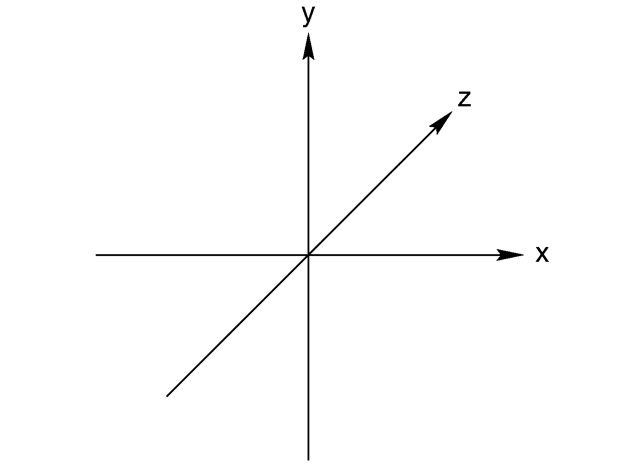
\includegraphics[scale=0.3]{handed.png}
\caption{Coordinate for 3D torus}
\end{figure}
Suppose the coordinate (x, y, z) is denoted as above (Figure 1). The root is at the origin. There are three phases for the broadcasting. In the first phase, the root sends messages to all the processes along the x-axis. Then, processes (i, 0, 0) send the messages to all processes (i, j, 0). At last, processes (i, j, 0) send the messages to processes (i, j, k), where $0 \le i, j, k \le \sqrt[3]{P}$. Each phase applies the ring broadcasting.
\begin{itemize}
\item Phase 1: $\frac{1}{3}\log_2P(t_s + m*t_w)+(\sqrt[3]{P} - 1)*t_h$
\item Phase 2: $\frac{1}{3}\log_2P(t_s + m*t_w)+(\sqrt[3]{P} - 1)*t_h$
\item Phase 3: $\frac{1}{3}\log_2P(t_s + m*t_w)+(\sqrt[3]{P} - 1)*t_h$
\end{itemize}
Therefore, the time complexity is $t_{comm} = \log_2P(t_s + m*t_w)+3(\sqrt[3]{P} - 1)*t_h$.
\item \textbf{Binary tree}\\[10pt]
There are $\log_2P$ steps in total. For each step, there are $2\log_2P$, $2\log_2P/2$,$\cdots$,$2\log_2(P/2^{\log_2P-1})$ hops, respectively. Therefore, the time complexity is
\begin{align*}
t_{comm} &= log_2P(t_s+m*t_w)+2(\log_2P+\log_2P/2+,...,+1)*t_h\\
&= log_2P(t_s+m*t_w)+ 2(\log_2P*\log_2P - (1+2+3+,...,+(\log_2P-1)))*t_h\\
&= log_2P(t_s+m*t_w) + \log_2P(\log_2P+1)*t_h
\end{align*}
\end{enumerate}
\section{Long message broadcasting}
\begin{enumerate}
\item \textbf{Ring}\\[10pt]
The time complexity for each algorithm is:
\begin{itemize}
\item One to all broadcasting in a ring: $\log_2P(t_s+M*t_w)$
\item New algorithm:\\[5pt] 
1. Scatter: $\log_2P*t_s+\frac{M}{P}*(P-1)*t_w$\\[5pt]
2. All to all broadcasting: $(P-1)(t_s+\frac{M}{P}*t_w)$
\end{itemize}
Therefore, to ensure the new algorithm is faster than the original algorithm,
\begin{equation*}
\log_2P*t_s+\frac{M}{P}*(P-1)*t_w + (P-1)(t_s+\frac{M}{P}*t_w) < \log_2P(t_s+M*t_w)
\end{equation*}
\begin{equation*}
M > \frac{P-1}{\log_2P+\frac{2}{P}-2}*\frac{t_s}{t_w}
\end{equation*}
\item \textbf{2-dimensional torus}\\[10pt]
Similarly, the time complexity for each algorithm is:
\begin{itemize}
\item One to all broadcasting in a 2D torus: $\log_2P(t_s+M*t_w)$
\item New algorithm:\\[5pt] 
1. Scatter: In Phase 1, the root scatters the message to one direction (say, to the nodes in row 0). Then in Phase 2, these nodes scatter the message to the other nodes in the column. \\[5pt]
\begin{itemize}
\item Phase 1: $\frac{1}{2}\log_2P*t_s+\frac{M}{\sqrt{P}}*(\sqrt{P}-1)*t_w$\\[5pt]
\item Phase 2: $\frac{1}{2}\log_2P*t_s+\frac{M}{P}*(\sqrt{P}-1)*t_w$\\[5pt]
\item Total: $\log_2P*t_s+ \frac{P-1}{P}*M*t_w$ \\[5pt]
\end{itemize}
2. Broadcasting: 
\begin{itemize}
\item Phase 1: all to all broadcast in every row like the ring algorithm $(\sqrt{P}-1)(t_s+\frac{M}{P}*t_w)$ \\[5pt]
\item Phase 2: similarly, all to all broadcast in every column $(\sqrt{P}-1)(t_s+\frac{M}{\sqrt{P}}*t_w)$ \\[5pt]
\item Total: $2(\sqrt{P}-1)*t_s+\frac{P-1}{P}*M*t_w$
\end{itemize}
\end{itemize}
Therefore, to ensure the new algorithm is faster than the original algorithm,
\begin{equation*}
\log_2P*t_s+ \frac{P-1}{P}*M*t_w + 2(\sqrt{P}-1)*t_s+\frac{P-1}{P}*M*t_w < \log_2P(t_s+M*t_w)
\end{equation*}
\begin{equation*}
M > \frac{2(\sqrt{P}-1)}{\log_2P+\frac{2}{P}-2}*\frac{t_s}{t_w}
\end{equation*}
\end{enumerate}
\end{document}
